% Created 2023-11-23 Do 09:41
% Intended LaTeX compiler: pdflatex
\documentclass[11pt]{article}
\usepackage[utf8]{inputenc}
\usepackage[T1]{fontenc}
\usepackage{graphicx}
\usepackage{longtable}
\usepackage{wrapfig}
\usepackage{rotating}
\usepackage[normalem]{ulem}
\usepackage{amsmath}
\usepackage{amssymb}
\usepackage{capt-of}
\usepackage{hyperref}
\author{Jeremy Sztavinovszki}
\date{\today}
\title{Collections Sztavinovszki}
\hypersetup{
 pdfauthor={Jeremy Sztavinovszki},
 pdftitle={Collections Sztavinovszki},
 pdfkeywords={},
 pdfsubject={},
 pdfcreator={Emacs 28.2 (Org mode 9.7)}, 
 pdflang={English}}
\usepackage{biblatex}

\begin{document}

\maketitle
\tableofcontents

\section{Funktionierender PL/SQL code.}
\label{sec:org5a9356d}
\begin{verbatim}
DECLARE
    l_names DBMS_UTILITY.maxname_array;
BEGIN
    l_names (1) := 'Strawberry';
    l_names (10) := 'Blackberry';
    l_names (2) := 'Raspberry';

    DECLARE
        indx PLS_INTEGER := l_names.FIRST;
    BEGIN

        WHILE (indx IS NOT NULL)
        LOOP
            DBMS_OUTPUT.put_line (l_names (indx));
            indx := l_names.NEXT (indx);
        END LOOP;
    END;
END;
/
\end{verbatim}
\section{Output}
\label{sec:org5fa0934}
\begin{center}
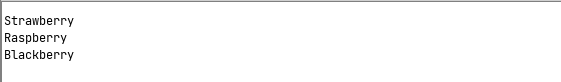
\includegraphics[width=.9\linewidth]{./output_pic.png}
\end{center}
\section{Erklärung}
\label{sec:org719fc05}
Das ist der richtige code, weil hier der Index in einem Block vor dem Loop deklariert und mit der   NEXT Anweisung aus dem Associative Array gefetched wird nach jeder Iteration.
In den anderen Beispielen gibt's entweder indx nicht definiert, oder es wird nicht/falsch gefetched.
\end{document}